\documentclass[a4paper, 11pt]{article}
\usepackage[catalan]{babel}
\usepackage[left=3cm,right=3cm,top=2cm,bottom=2cm]{geometry}
\usepackage{parskip}
\usepackage{biblatex, csquotes}
\usepackage{amsmath, amssymb}
\usepackage{float, graphicx}
\usepackage{bookmark}

\addbibresource{l03.bib}

\hypersetup{
  colorlinks=true,
  citecolor=magenta,
  linkcolor=blue,
  urlcolor=cyan,
  pdftitle={Interpretació geomètrica de YBC6967},
  pdfpagemode=FullScreen,
}

\title{\textit{The Newton Project}, un repte majúscul.}
\author{
  Carlo Sala Gancho\\
  Història de les Matemàtiques\\
  Grau de Matemàtiques\\
  Universitat Autònoma de Barcelona}

\date{Març 2023}

\begin{document}

\maketitle

\subsection*{L'aversió a la publicació}

Sir Isaac Newton és un dels matemàtics i físics (i qui sap quantes ciències més) més grans de tots els temps, d'això no
hi ha ni tan sols una espurna de dubte. Ara bé, ens pot arribar a sorpendre una característica seva: no sempre
publicava la seva feina. Per exemple, durant els seus \textit{Anni mirabilis} (1665/1666) va crear (o descobrir) el
càlcul, i va escriure'n un tractat durant l'any 1671, però no va ser publicat fins al 1736, una dècada després de la
seva mort.~\cite{bib:methodfluxions} Exemples com aquests no són excepcionals quan es revisa l'obra de Newton.

Aquesta certa aversió, raons de la qual no seran el focus principal d'aquest text, porta al fet que recopilar tots els
escrits i tractats del matemàtic anglès tingui encara més dificultats que les pròpies de buscar i digitalitzar
manuscrits de fa més de 300 anys.

\subsection*{El naixement de \textit{The Newton Project}~\cite{bib:newtonproject}}

Dirigit per Rob Iliffe i Scott Mandelbrote des de la universitat d'Oxford, al Regne Unit, el projecte neix a l'any 1998
amb l'objectiu de recopilar, digitalitzar, normalitzar i enriquir els textos no científics\footnotemark{} de Newton.
L'objectiu de crear una edició exhaustiva d'aquest subconjunt de textos de Newton sembla, a primera vista, summament
inabastable. No satisfets amb aquesta fita, l'any 2007 va decidir ampliar el seu camp de visió per perseguir l'objectiu
d'editar la totalitat de textos de Newton, ja siguin publicats, no publicats, cartes manuscrites, etc. Actualment, més
del 95\% de textos no científics han estat introduits satisfactòriament dins del sistema, i hi ha un total de 1911
obres publicades.

\footnotetext{Els autors del projecte, posen entre cometes les paraules \textit{no científics}. D'alguna manera, és
  difícil saber què es considera una ciència i què no. Per exemple, la teologia era considerada una ciència, i fins i tot
  una branca de les ciències naturals amb la teologia natural, que es va desenvolupar molt a finals de segle XVII i el
  segle XVIII.}

\subsection*{Els reptes tècnics}

La producció matemàtica de Newton va ser immensa i, a més, molt heterogènia en quant a formats. Molts dels seus
tractats i raonaments ens arriben a través de cartes enviades a co\lgem{}gues a través de la secretaria de la Societat
Reial de Londres, un organisme clau pels científics de l'època.

Per aconseguir-ho, el projecte fa ús dels \textit{frameworks} de codificació MathML i TEI-P5. Els dos són estàndars
oberts, i les seves especificacions i software són totalment software lliure. A més, els investigadors que n'estiguin
estudiant els textos, poden veure l'historial de modificacions que han anat acumulant cada un dels textos, i els
usuaris més avançats poden també veure'n el codi XML que compon els textos. En definitiva, es tracta d'una feina molt
conscient amb el lliure estudi i distribució dels textos del matemàtic britànic, sempre donant la màxima informació
possible. La majoria de textos es poden consultar traduits a l'anglès i transcrits en la llengua original (llatí,
majoritàriament), a més d'imatges del manuscrit original.

El fet de centralitzar i normalitzar tots els textos a una mateix estàndard es tracta d'un dels reptes més grans que
afronta el projecte, i requereix de milers d'hores d'investigadors per cada petita porció de text.

\begin{figure}[H]
  \centering
  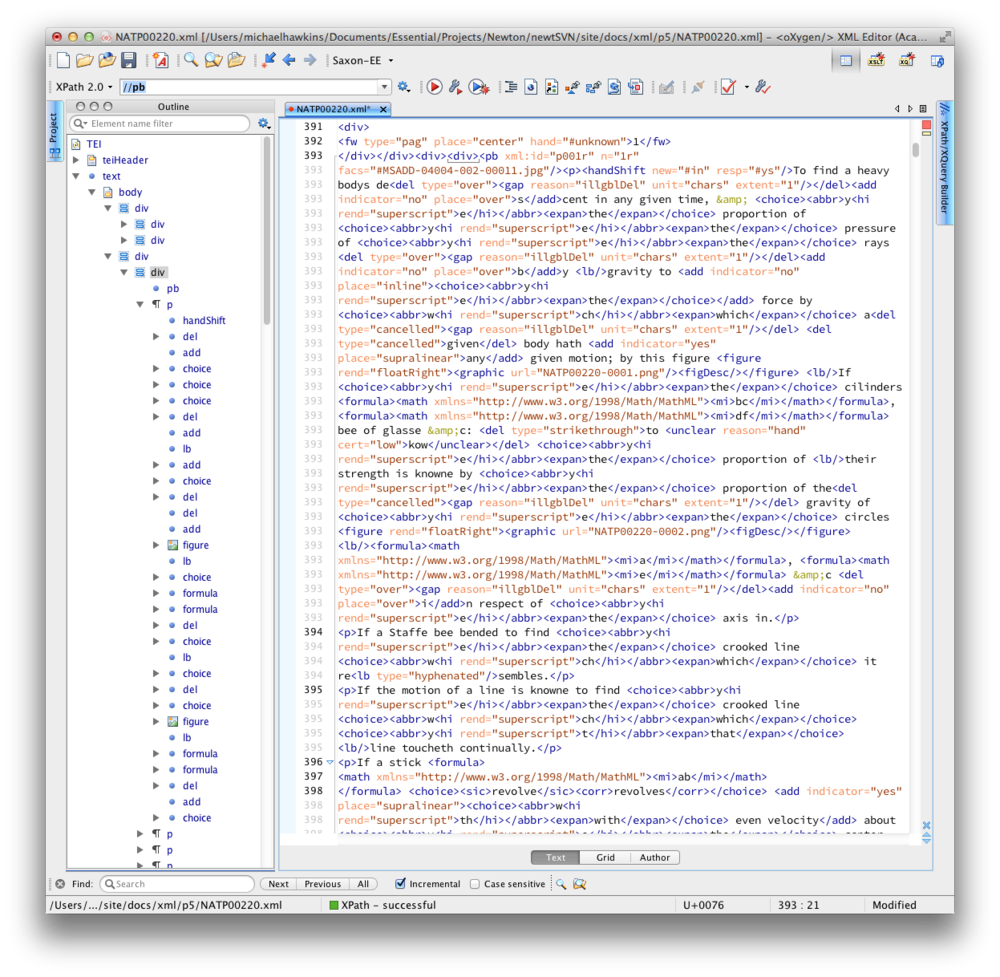
\includegraphics[width=10cm]{exemple-newtonproject.png}
  \caption{Exemple de text matemàtic codificat amb MathML.~\cite{bib:fig:exemple}}
\end{figure}

\subsection*{Una iniciativa única}

L'esforç que l'equip de \textit{The Newton Project} està posant en impulsar fins a la sacietat l'edició dels textos de
Newton és realment increïble. Sovint sentim comentaris al carrer que els historiadors no tenen feina, que està tot
investigat. Descobrint projectes com aquest, notem que la història, i en particular la història de la ciència, viuen un
moment brillant de la seva, valgui la redundància, història: la digitalització i binarització de tota la quantitat
ingent de dades que, fins ara, només trobàvem al paper, obre tot un ventall de noves possibilitats d'estudi fins ara
impensables. Calen més iniciatives com aquesta en altres àmbits per seguir aprenent d'aquells que ens van precedir.

\printbibliography{}
\end{document}
